\begin{frame}{Systèmes complexes}
  \begin{block}{Système complexe}
    Un système complexe est un ensemble constitué d'un grand nombre d'entités en interaction qui empêchent l'observateur de prévoir sa rétroaction, son comportement ou évolution par le calcul.
  \end{block}
  \pause
  \begin{exampleblock}{Exemples}
    \begin{itemize}
    \item programmes informatiques
    \item protocoles de sécurité
    \item circuits logiques
    \end{itemize}
  \end{exampleblock}
\end{frame}

\begin{frame}{Le génie logiciel}
  \begin{columns}
    \begin{column}{0.6\textwidth}
      \begin{center}
        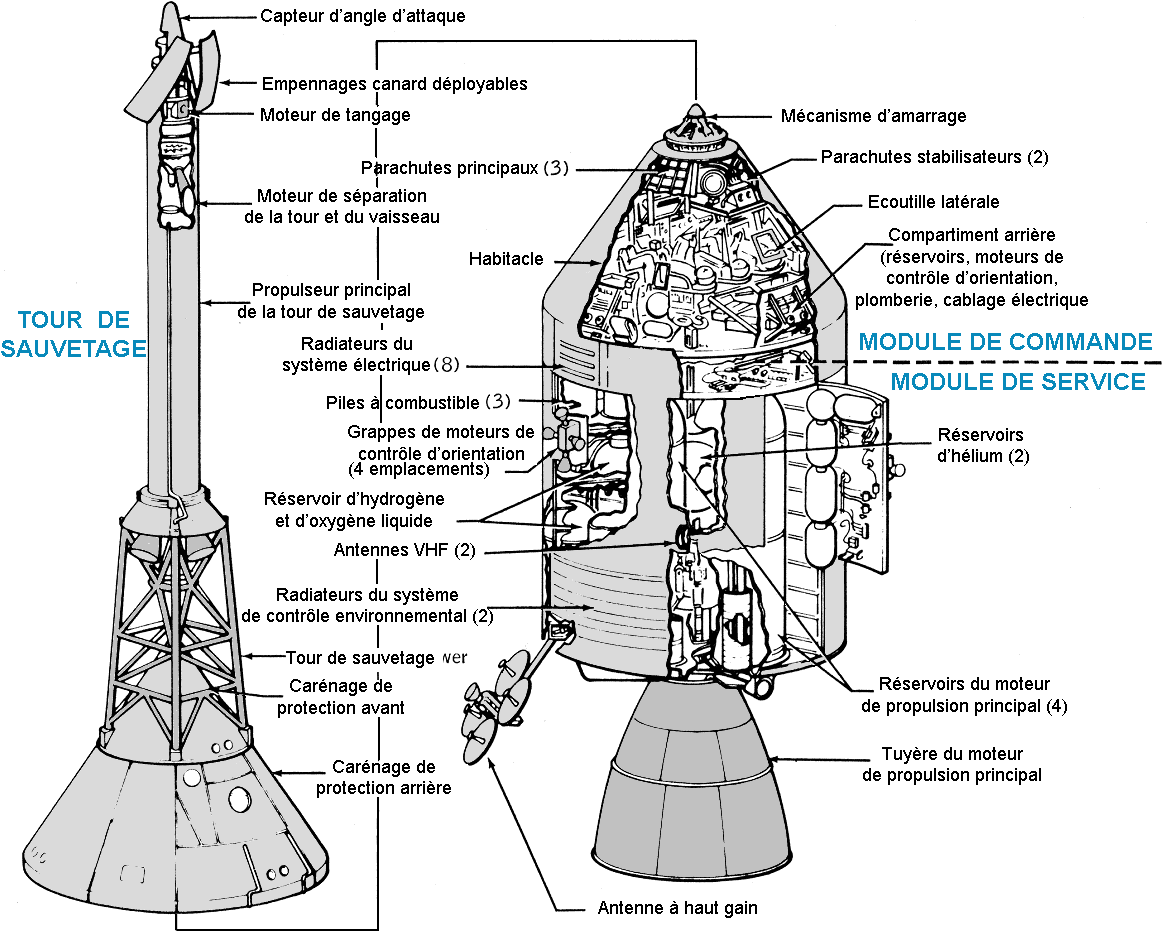
\includegraphics[height=4cm]{media/apollo.png}
      \end{center}
      \onslide<2>
      \begin{block}{Génie logiciel}
        L'ensemble des activités de conception et de mise en œuvre des produits et des procédures tendant à rationaliser la production du logiciel et son suivi.
      \end{block}
    \end{column}
    \begin{column}{0.4\textwidth}
      \onslide<1->
      \begin{center}
        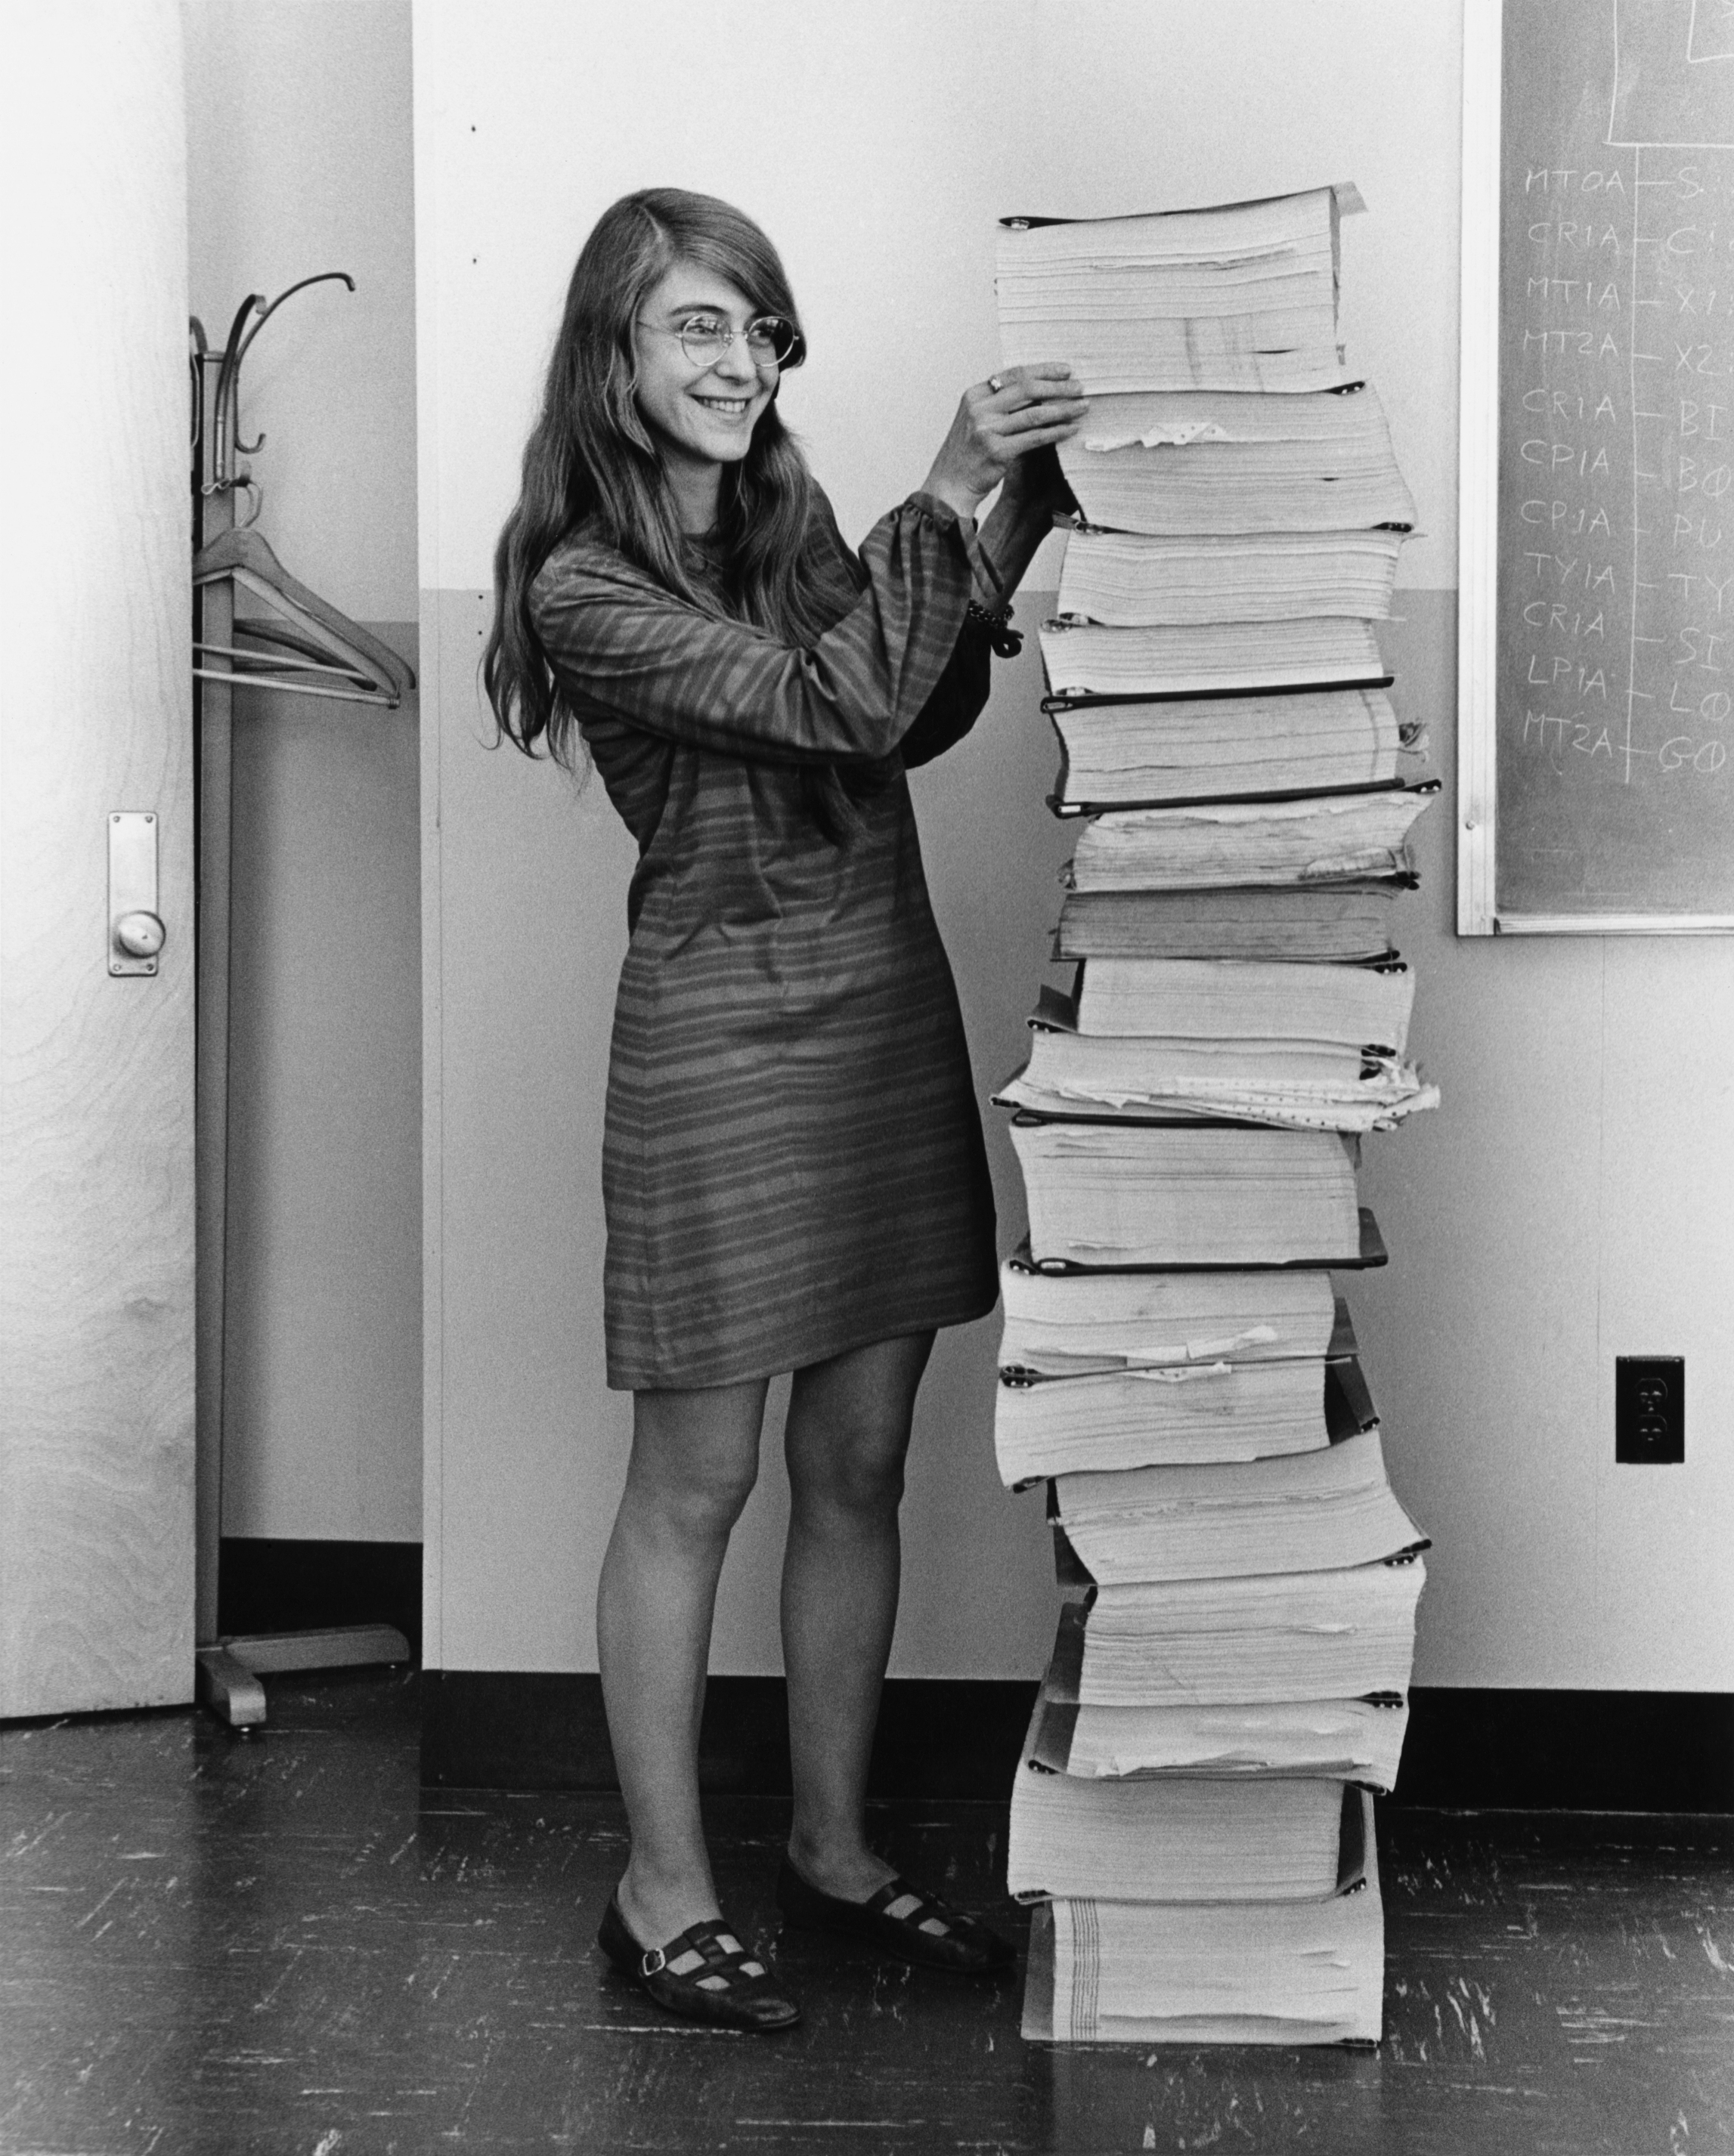
\includegraphics[width=0.9\textwidth]{media/MHamilton.jpg}
      \end{center}
    \end{column}
  \end{columns}
\end{frame}

\begin{frame}{Vérification}
  Conformité et fiabilité d'un système complexe ?
  \pause
  \begin{block}{}
    \begin{itemize}[<+->]
    \item Les tests
      \begin{itemize}
      \item si l'ensemble d'entrées est trop grand ou infini ?
      \end{itemize}
    \item Les méthodes formelles
      \begin{itemize}
      \item analyse statique par interprétation abstraite
      \item vérification déductive
      \item vérification de modèles
      \end{itemize}
    \end{itemize}
  \end{block}
\end{frame}

\begin{frame}{Analyse statique par interprétation abstraite}
  \begin{columns}
    \begin{column}{0.3\textwidth}
      \begin{center}
        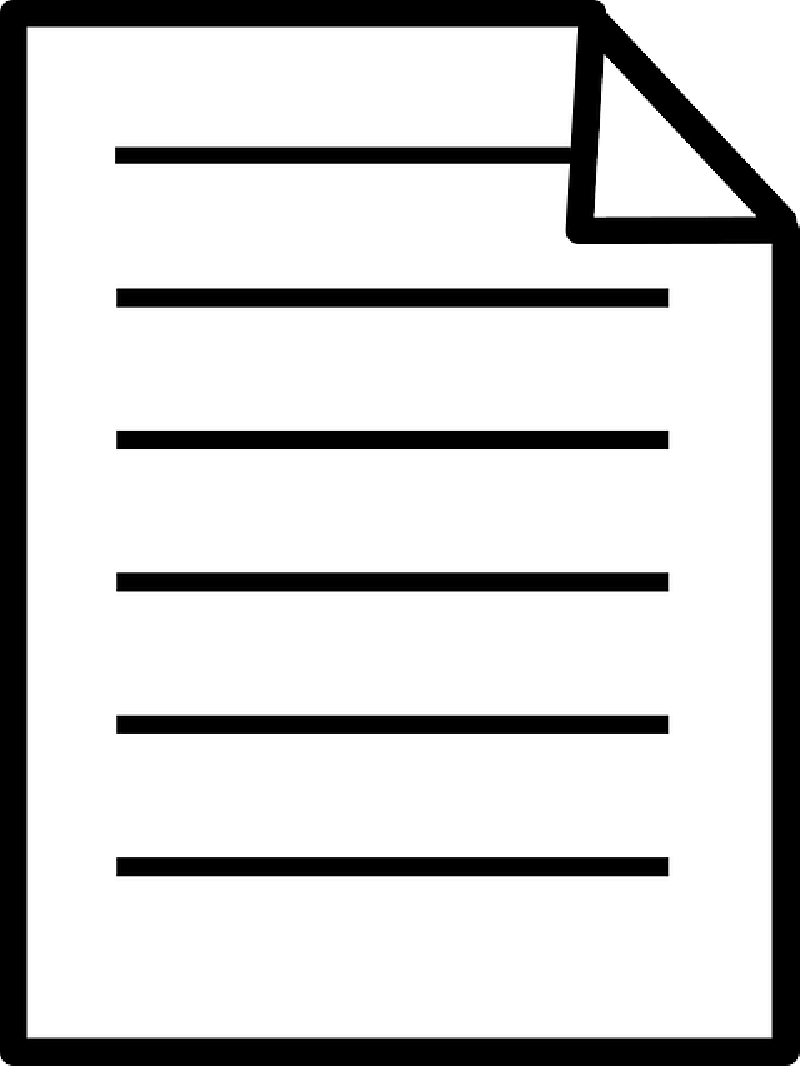
\includegraphics[width=0.5\textwidth]{media/fichier.png}
        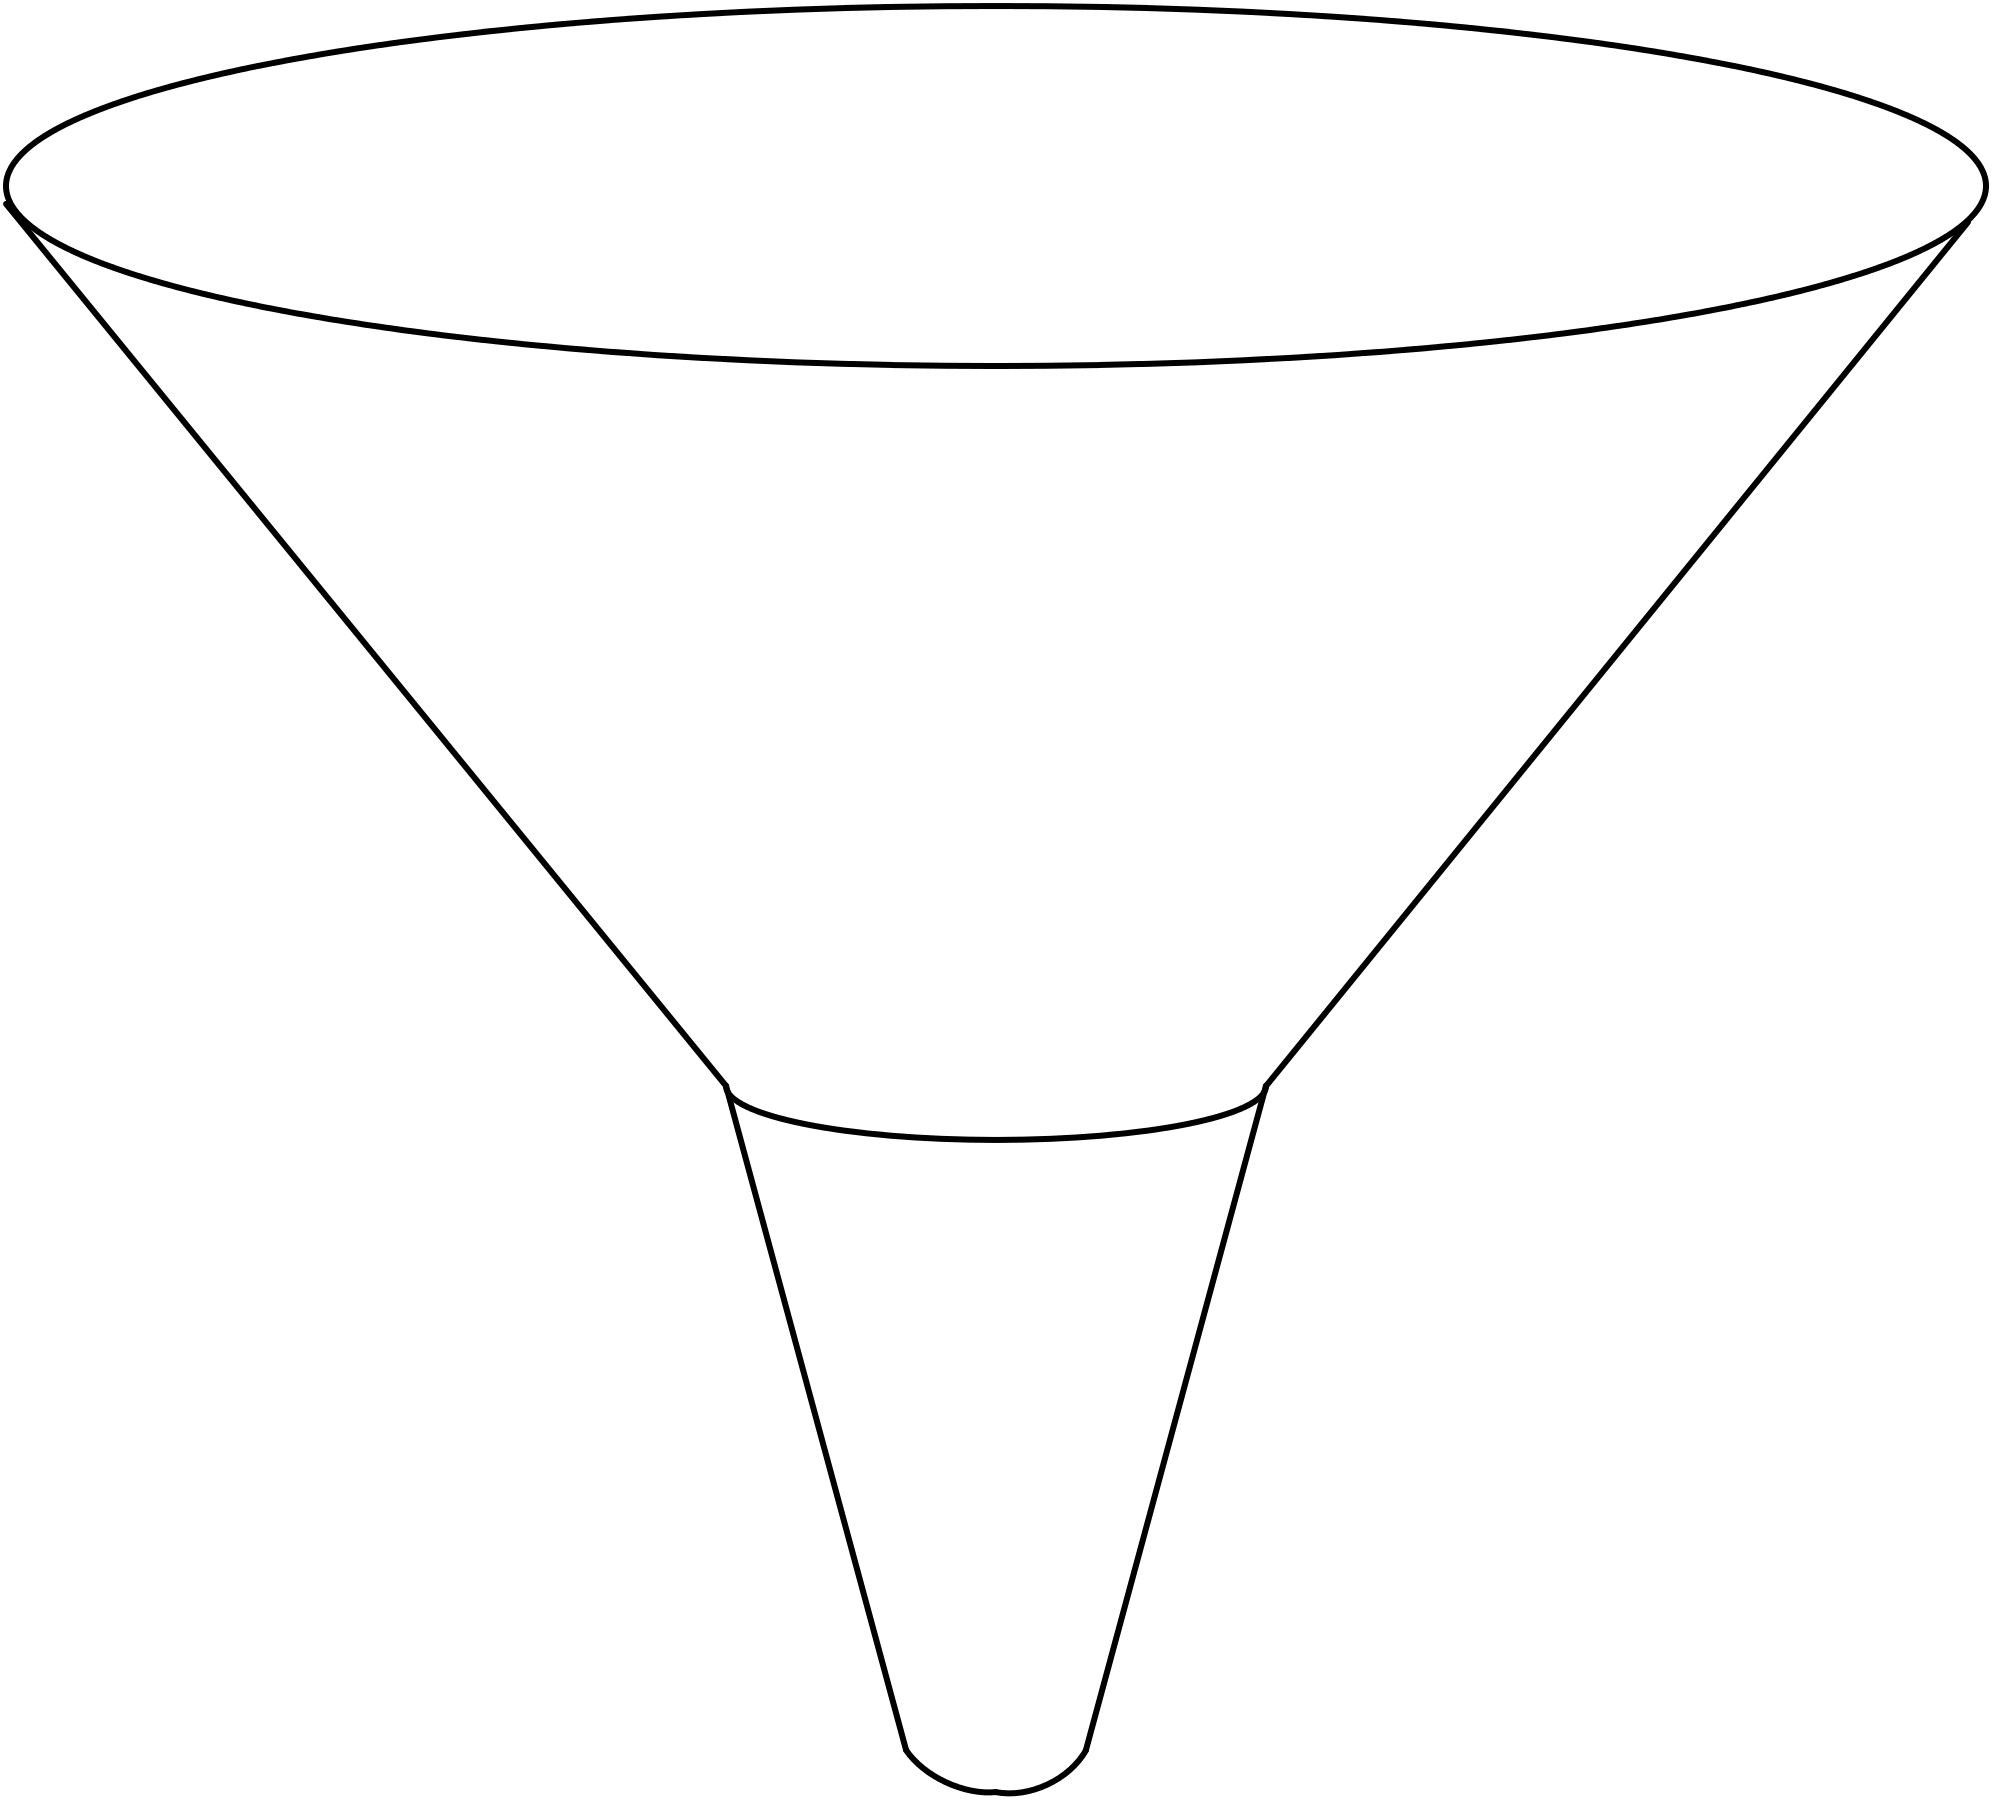
\includegraphics[width=\textwidth]{media/entonnoir.png}
        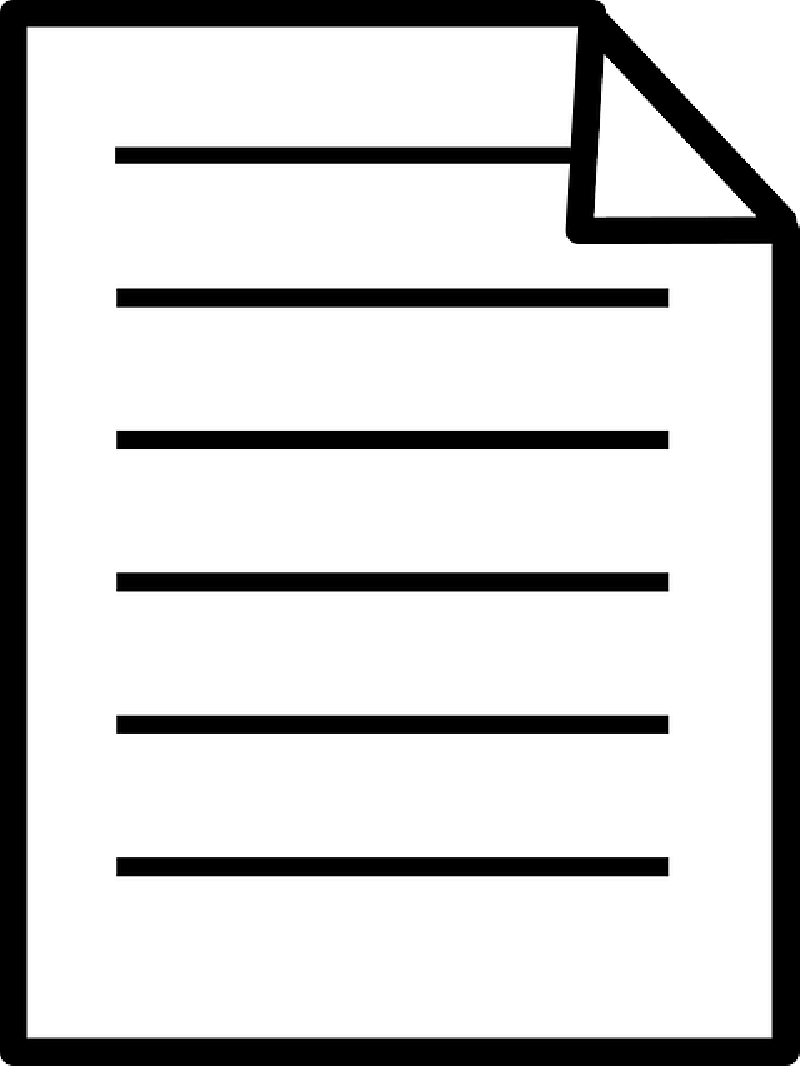
\includegraphics[width=0.25\textwidth]{media/fichier.png}
      \end{center}
    \end{column}
    \begin{column}{0.5\textwidth}
      \begin{block}{}
        \begin{itemize}
        \item Constat
          \begin{itemize}
          \item trop d'informations
          \end{itemize}
        \item Solution
          \begin{itemize}
          \item utilisation d'abstractions
          \end{itemize}
        \item Difficulté
          \begin{itemize}
          \item garder suffisamment d'informations
          \item mais pas trop
          \end{itemize}
        \end{itemize}
      \end{block}
    \end{column}
  \end{columns}
\end{frame}

\begin{frame}{Vérification déductive}
  \begin{overprint}
    \begin{tikzpicture}
      
      \tikzstyle{domino} = [minimum width=1.7cm, minimum height=1cm, draw]
      \tikzstyle{dependancy} = [->, thick]
      
       \onslide<1->{
         \node (shredder) at (0,1.5) {
\includegraphics[width=0.3\textwidth]{media/shredder.png}};
       }

      \onslide<2->{
        \node[circle, minimum size=0.5cm, very thick, fill=white, draw] (small) at (0,0.4) {};
        \node[circle, minimum size=7cm, very thick, draw] (big) at (6,-0.5) {};
      
        \node[domino] (dom3pre) at (6, -2) {\tiny{préconditions}};
        \node[domino, below=0 of dom3pre] (dom3post) {\tiny{postconditions}};
        
        \draw[very thick] (small) -- (big);
      }
      
      \onslide<3->{
        \node[domino] (dom1pre) at (4.75, 1.25) {\tiny{préconditions}};
        \node[domino, below=0 of dom1pre] (dom1post) {\tiny{postconditions}};
      
        \node[domino] (dom2pre) at (7.25, 1.25) {\tiny{préconditions}};
        \node[domino, below=0 of dom2pre] (dom2post) {\tiny{postconditions}};
      
        \draw[dependancy] (dom1post.south) |- (5.5,-0.75) -- (dom3pre.134);
        \draw[dependancy] (dom2post.-134) |- (6.5,-0.75) -- (dom3pre.46);
        \draw[dependancy] (dom2post.-46) |- (8.25,-0.75) -- (8.25,2) -| (dom2pre.46);
        
        \draw[dependancy] (big.66) -| (dom2pre.134);
        \draw[dependancy] (big.north) -- (6,2.5 ) -| (dom1pre.north);
      }
    \end{tikzpicture}
  \end{overprint}
\end{frame}

\begin{frame}{Vérification de modèles}
  \begin{block}{}
    \begin{itemize}
    \item Analyse exhaustive
    \item Représentation astucieuse
    \end{itemize}
  \end{block}
  \begin{columns}
    \begin{column}{0.5\textwidth}
      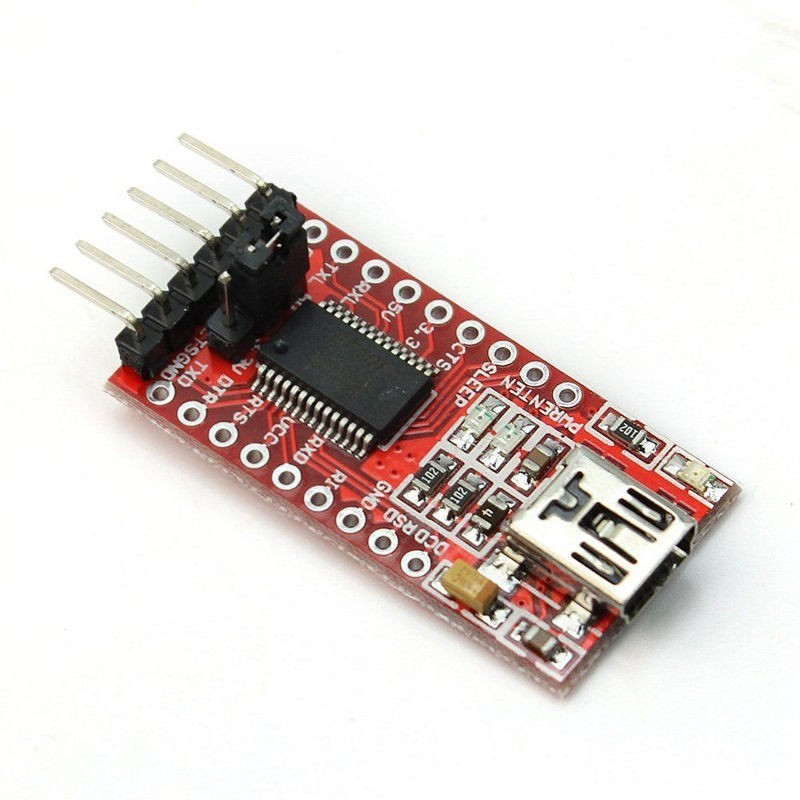
\includegraphics[width=\textwidth]{media/ftdi.jpg}
    \end{column}
    \begin{column}{0.5\textwidth}
      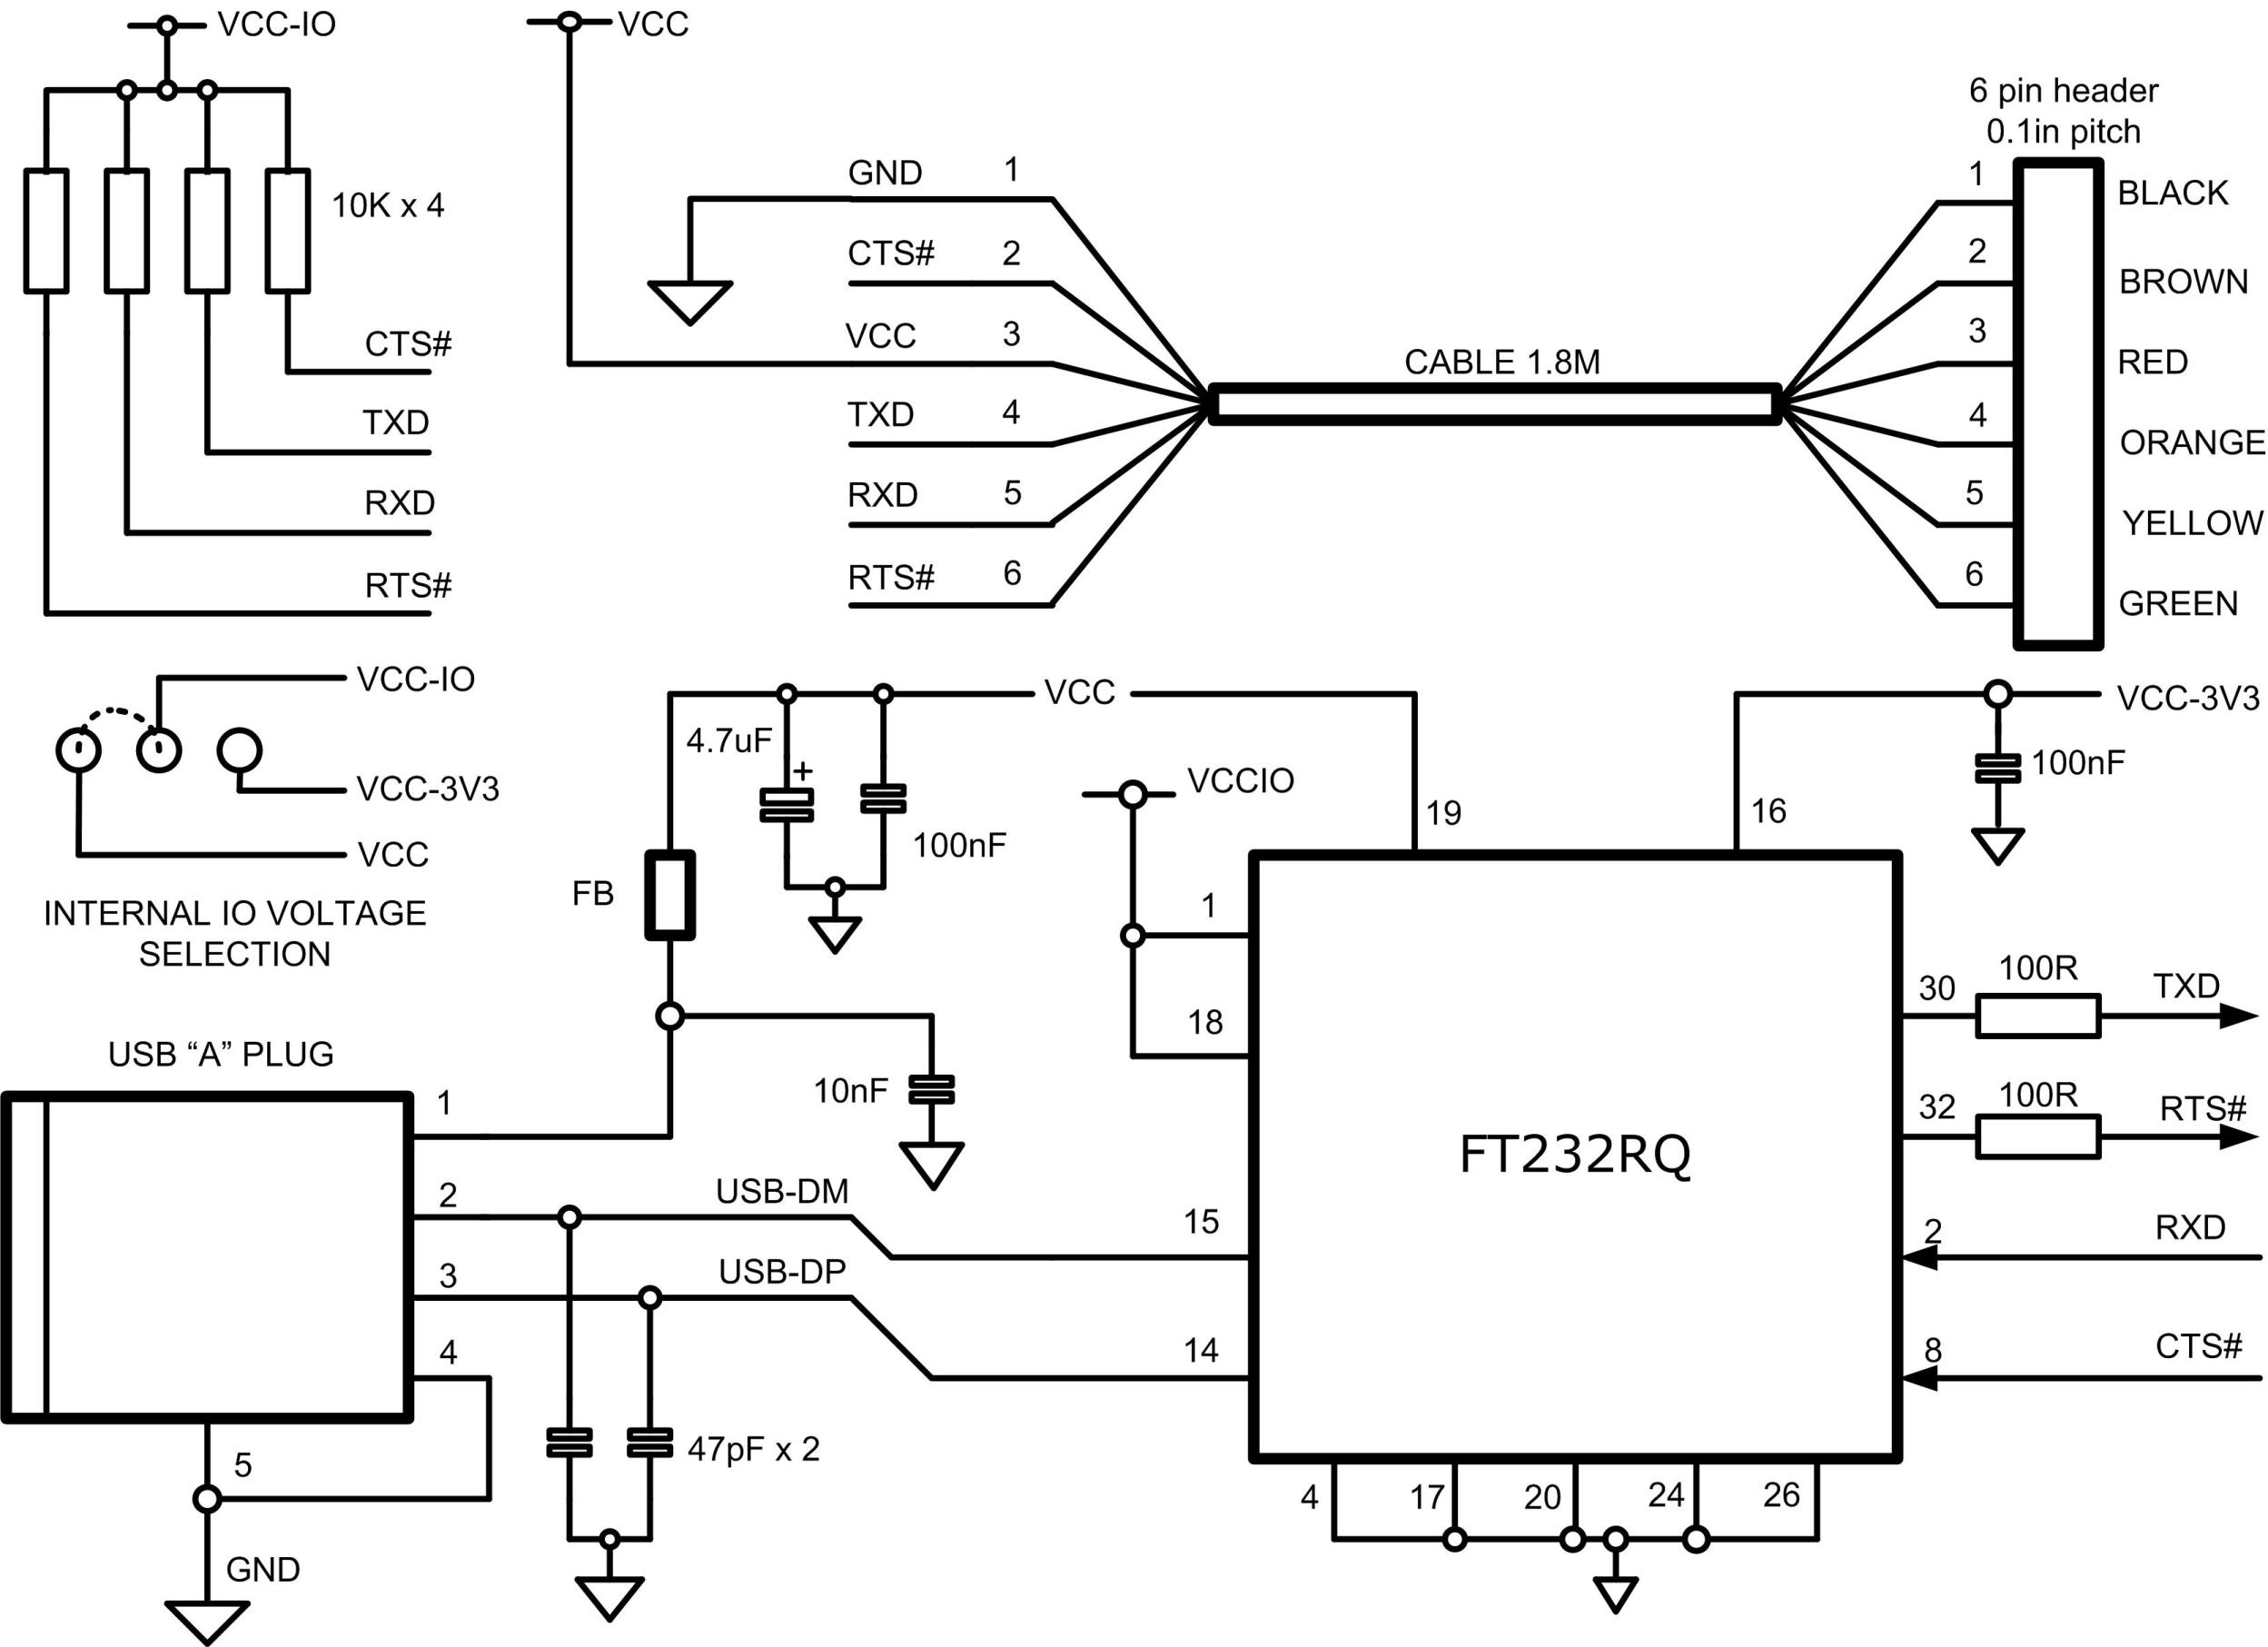
\includegraphics[width=\textwidth]{media/sftdi.jpg}
    \end{column}
  \end{columns}
\end{frame}

